 
\section{Search strategy for the charged Higgs at 13 TeV}
\label{s:searchStrategy}

The search for the charged Higgs boson in the $c\bar{s}$ channel at 13 \TeV 
in the CMS experiment adopted a similar strategy as that of the previous analysis
at 8 \TeV \cite{Khachatryan:2015uua}. An additional charm quark tagging have been
further exploited to improve sensitivity. The invariant mass of the jets originating from 
charm and strange antiquark is taken as the observable for the search of charged Higgs, in the 
low mass region from 80 to 160 \GeV. In the absence of an excess in the observed data,
a 95\% CL limit is put on the \brThb. The charm tagging is extensively used to
improve this limit. As shown on the right side of the Figure~\ref{fig:feyn_diag_sig}, 
for the signal process, one \PQt quark decays to $H^+ b$ and the other one to 
$W^- \bar{b}$. The $W^+/H^+$ decays hadronically, whereas the $W^-$ decays 
leptonically. As a result, in the final states, there are four jets (2 \PQb jets, 
1 \PQc jet, 1 \PQs jet), one lepton (electron or muon, $\tau$ is not considered) 
and missing transverse energy attributed to neutrino. In this thesis, we assume that the \brHcs =100\%.
\begin{figure}
\centering
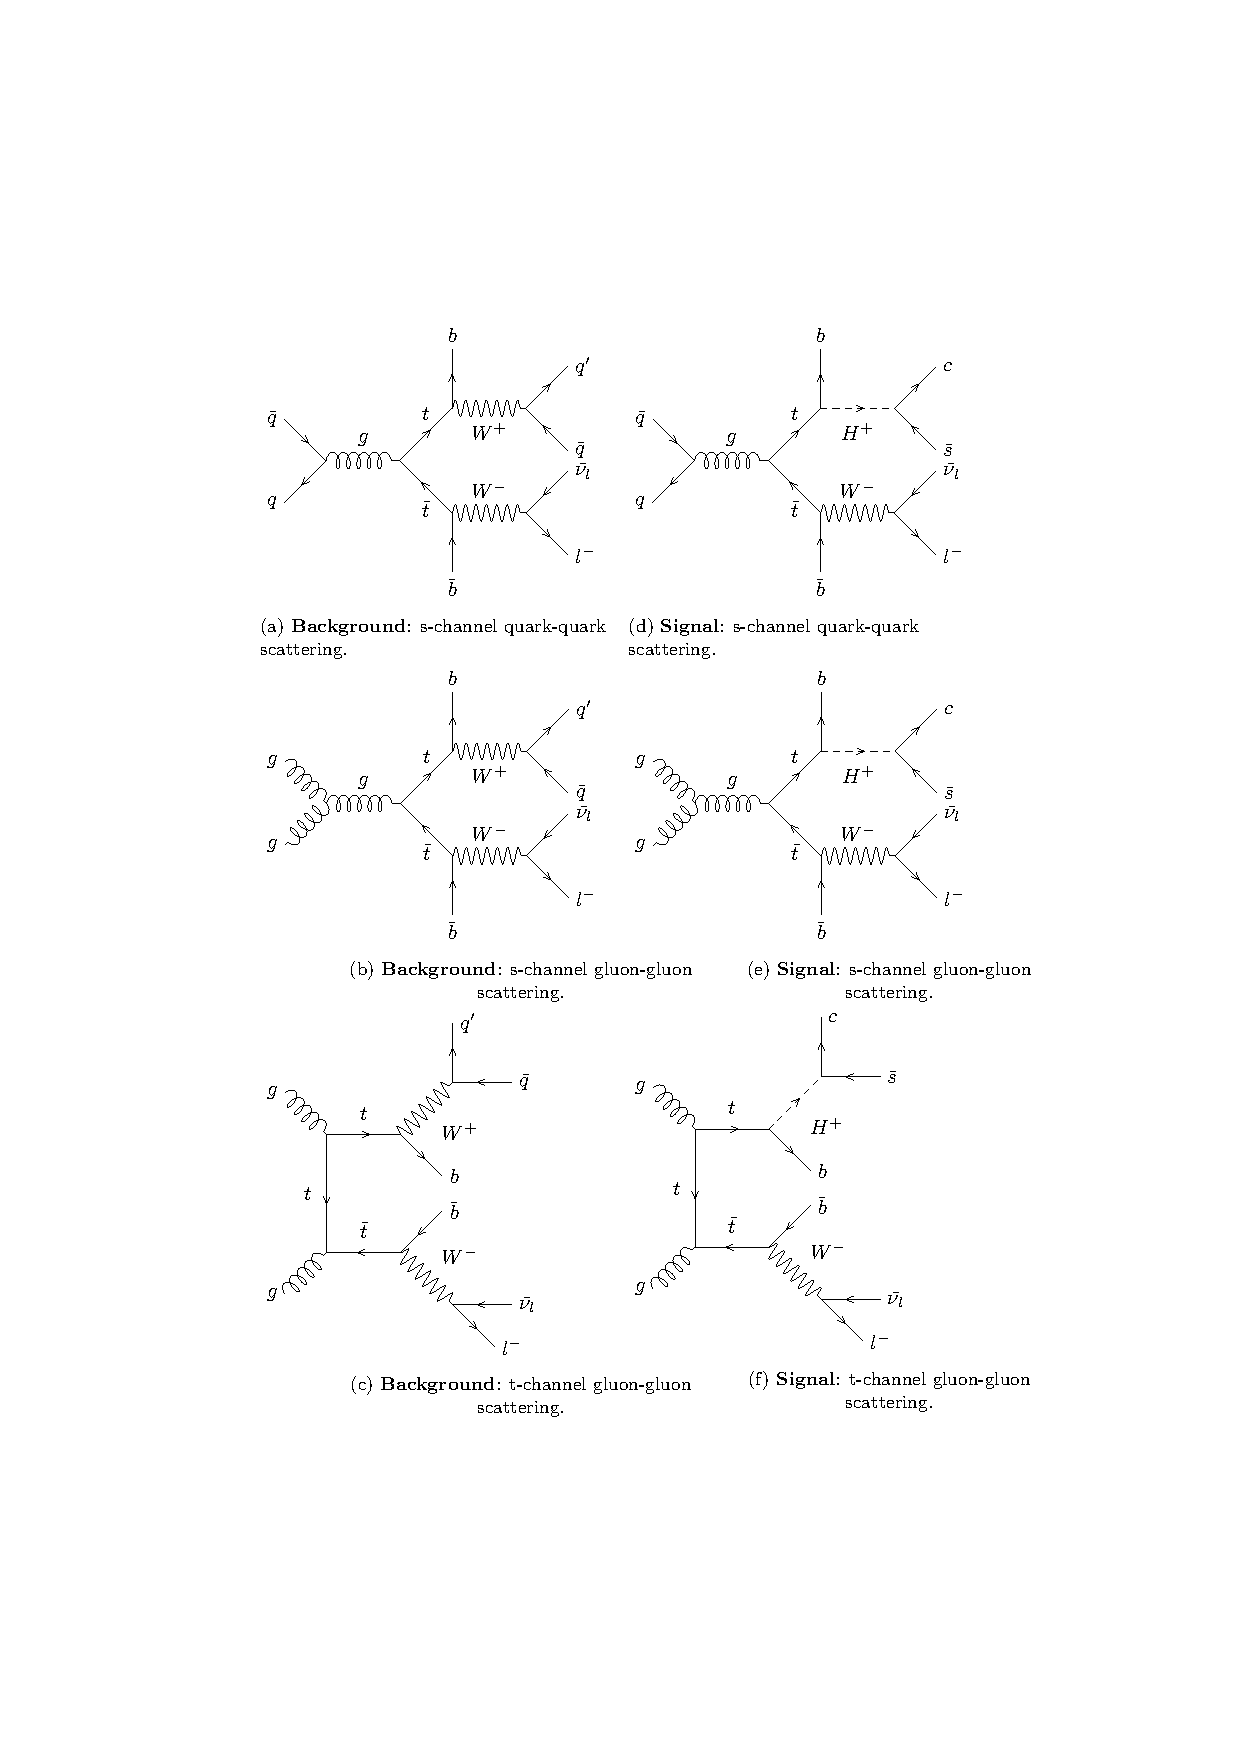
\includegraphics[width=0.75\textwidth]{Image/FeynDiag/feyn_diag_sig.pdf}
\caption{Production of \ttbar from gluon-gluon and quark-quark scattering. 
         The quark-scattering production process has a dominant contribution at 
         Tevatron energies whereas gluon-gluon scattering diagrams are dominant 
         at LHC energies ~\cite{Gerber:2014xea, Fiorini:2012fe}. The SM production
         of \ttbar is shown in (a), (b) and (c). The charged Higgs boson 
         production and its decay are shown in (d), (e), and (f).}
\label{fig:feyn_diag_sig}
\end{figure}

The standard Model processes that give same final states (4 jets + 1 lepton + missing 
energy) are considered as backgrounds for this analysis. The standard model
\ttbar production is the most dominant, irreducible background process. 
As shown in the left side of the Figure~\ref{fig:feyn_diag_sig}, for
SM \ttbar process, one \PQt quark decays to the $W^+$ and \PQb quark 
($t\rightarrow W^+ b$) and the other decays to $W^- \bar{b}$ 
($\bar{t}\rightarrow W^-\bar{b}$). The SM \ttbar contributes around 94\%
of the total backgrounds. Other sub-dominant backgrounds that give rise to similar 
final states are single \PQt quark production, QCD multijet, \wjets, \dyjets, 
and vector boson pair production processes. The following background processes are considered
for the search for charged Higgs. They are ordered in their significance of contribution.
\begin{enumerate}[leftmargin=*]
\item $\textbf{SM \ttjets}$: Feynman diagrams 
	for \ttjets production are shown on the left hand side of Figure
	\ref{fig:feyn_diag_sig}. This is the most dominant background channel
	in the signal search region (SR).

\item {\bf{Single \PQt}}: The single \PQt quark production process can also mimic the signal 
	topology. Three different ways, as shown in Figure~\ref{fig:feyn_diag_st}, 
	of production of single top quark considered in this analysis. It is produced through 
	s-channel, t-channel, and tW-channel. In the s-channel and t-channel the initial quarks 
	can be \PQu, \PQd, \PQc and \PQs (4-flavour scheme). However, in the tW-channel, 
	the initial quark is only \PQb quark (5-flavor scheme).
	\begin{figure}
	\begin{center}
	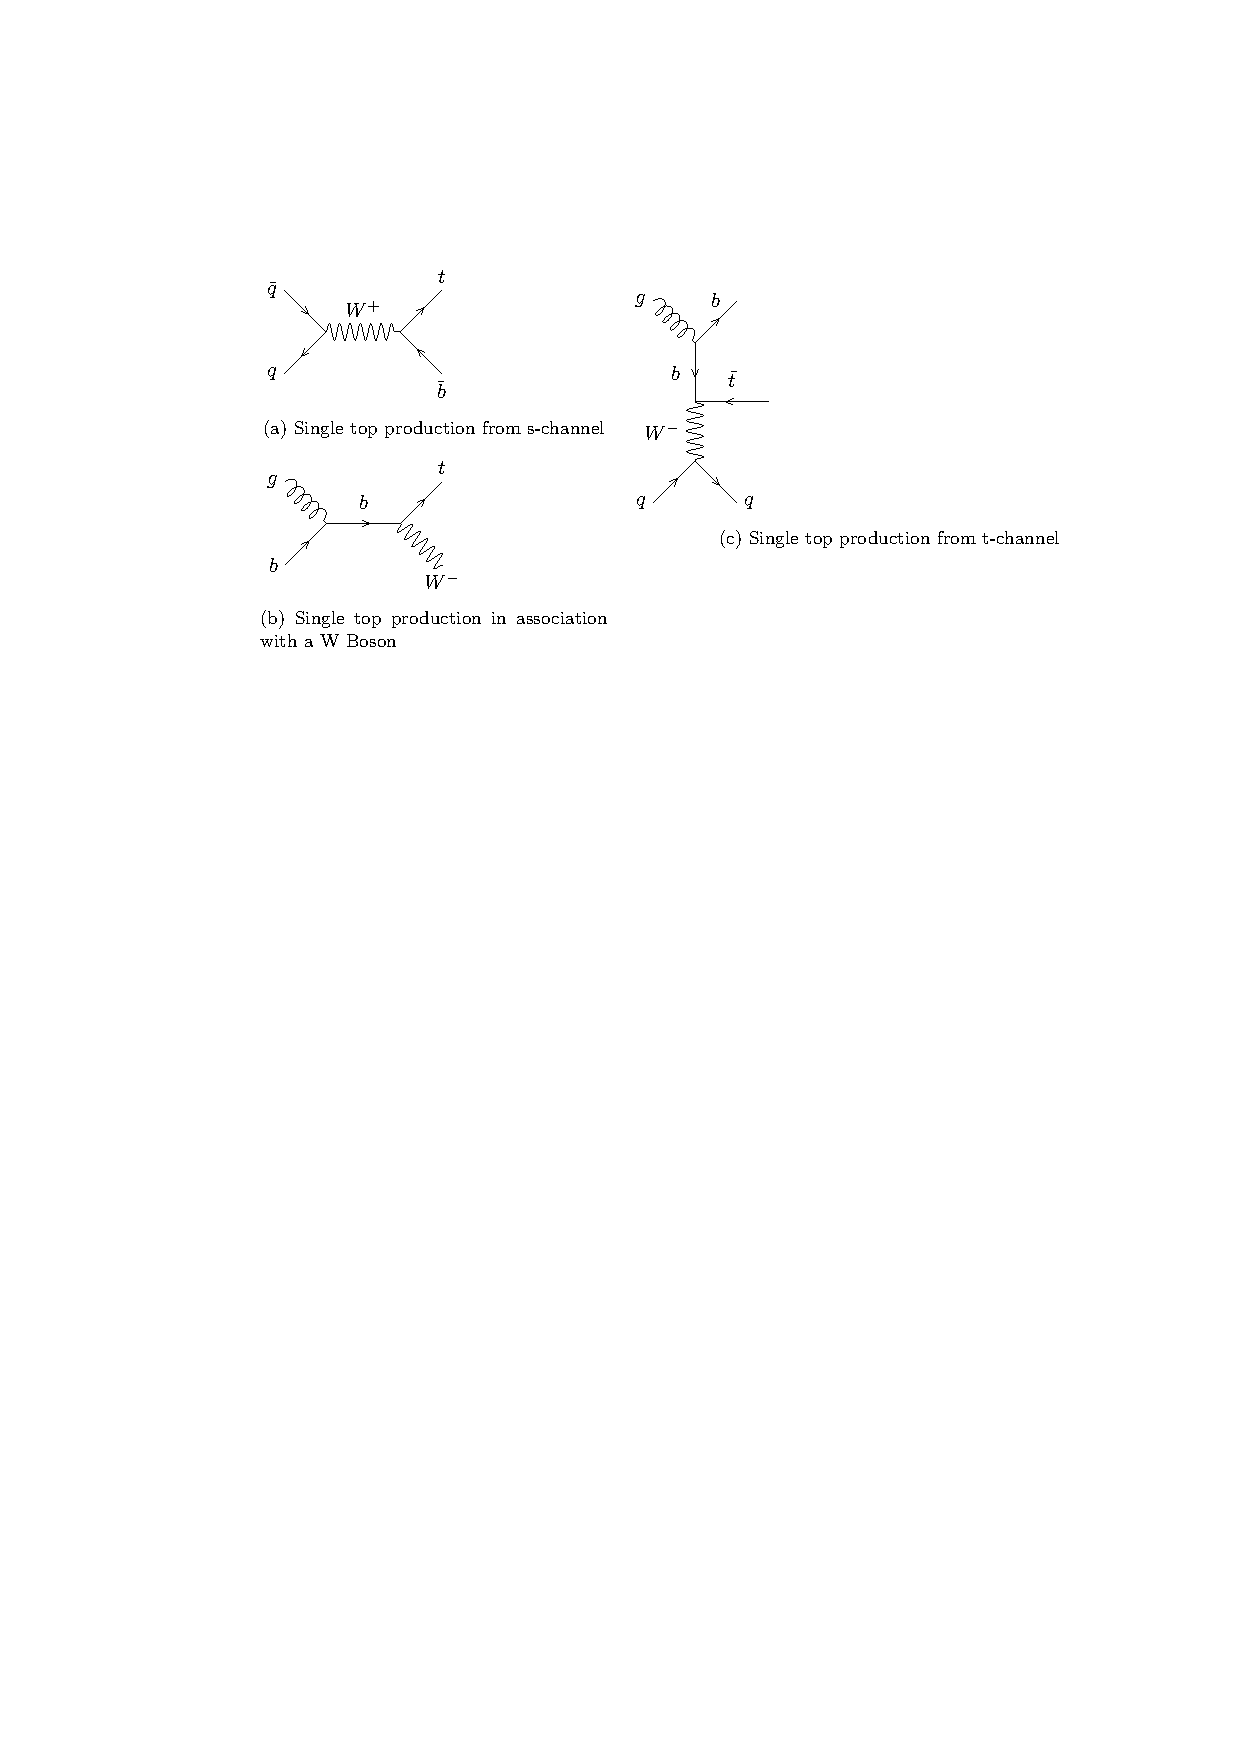
\includegraphics[width=0.75\textwidth]{Image/FeynDiag/feyn_diag_st.pdf}
	\caption{Representative Feynman diagrams for single \PQt quark production processes.}
	\label{fig:feyn_diag_st}
	\end{center}
	\end{figure}

\item {\bf{QCD multijet}}: The QCD multijet events contain only jets at parton level. However, after
	event reconstruction, they can still have leptons from misidentifications, and \MET due to 
	poor measurement of energy in the detector. Thus these events also mimic the signal topology.

\item {\bf{\wjets}}: In this process, a \PW boson is produced in the proton-proton 
	collisions which subsequently decays leptonically. Following \wjets 
	background process are considered in this analysis:
  	\begin{enumerate}[leftmargin=*]
  	  \item $\PW + \rm{jets  }(\PW^\pm \rightarrow l^+ \nu (l^-\bar{\nu}))$
  	  \item $\PW + \rm{1 jet }(\PW^\pm \rightarrow l^+ \nu (l^-\bar{\nu}))$
  	  \item $\PW + \rm{2 jets }(\PW^\pm \rightarrow l^+ \nu (l^-\bar{\nu}))$
  	  \item $\PW + \rm{3 jets }(\PW^\pm \rightarrow l^+ \nu (l^-\bar{\nu}))$
  	  \item $\PW + \rm{4 jets }(\PW^\pm \rightarrow l^+ \nu (l^-\bar{\nu}))$
  	\end{enumerate} 
	The Feynman diagram for these processes are shown in Figure~\ref{fig:feyn_diag_wjet}.
	\begin{figure}
	\begin{center}
	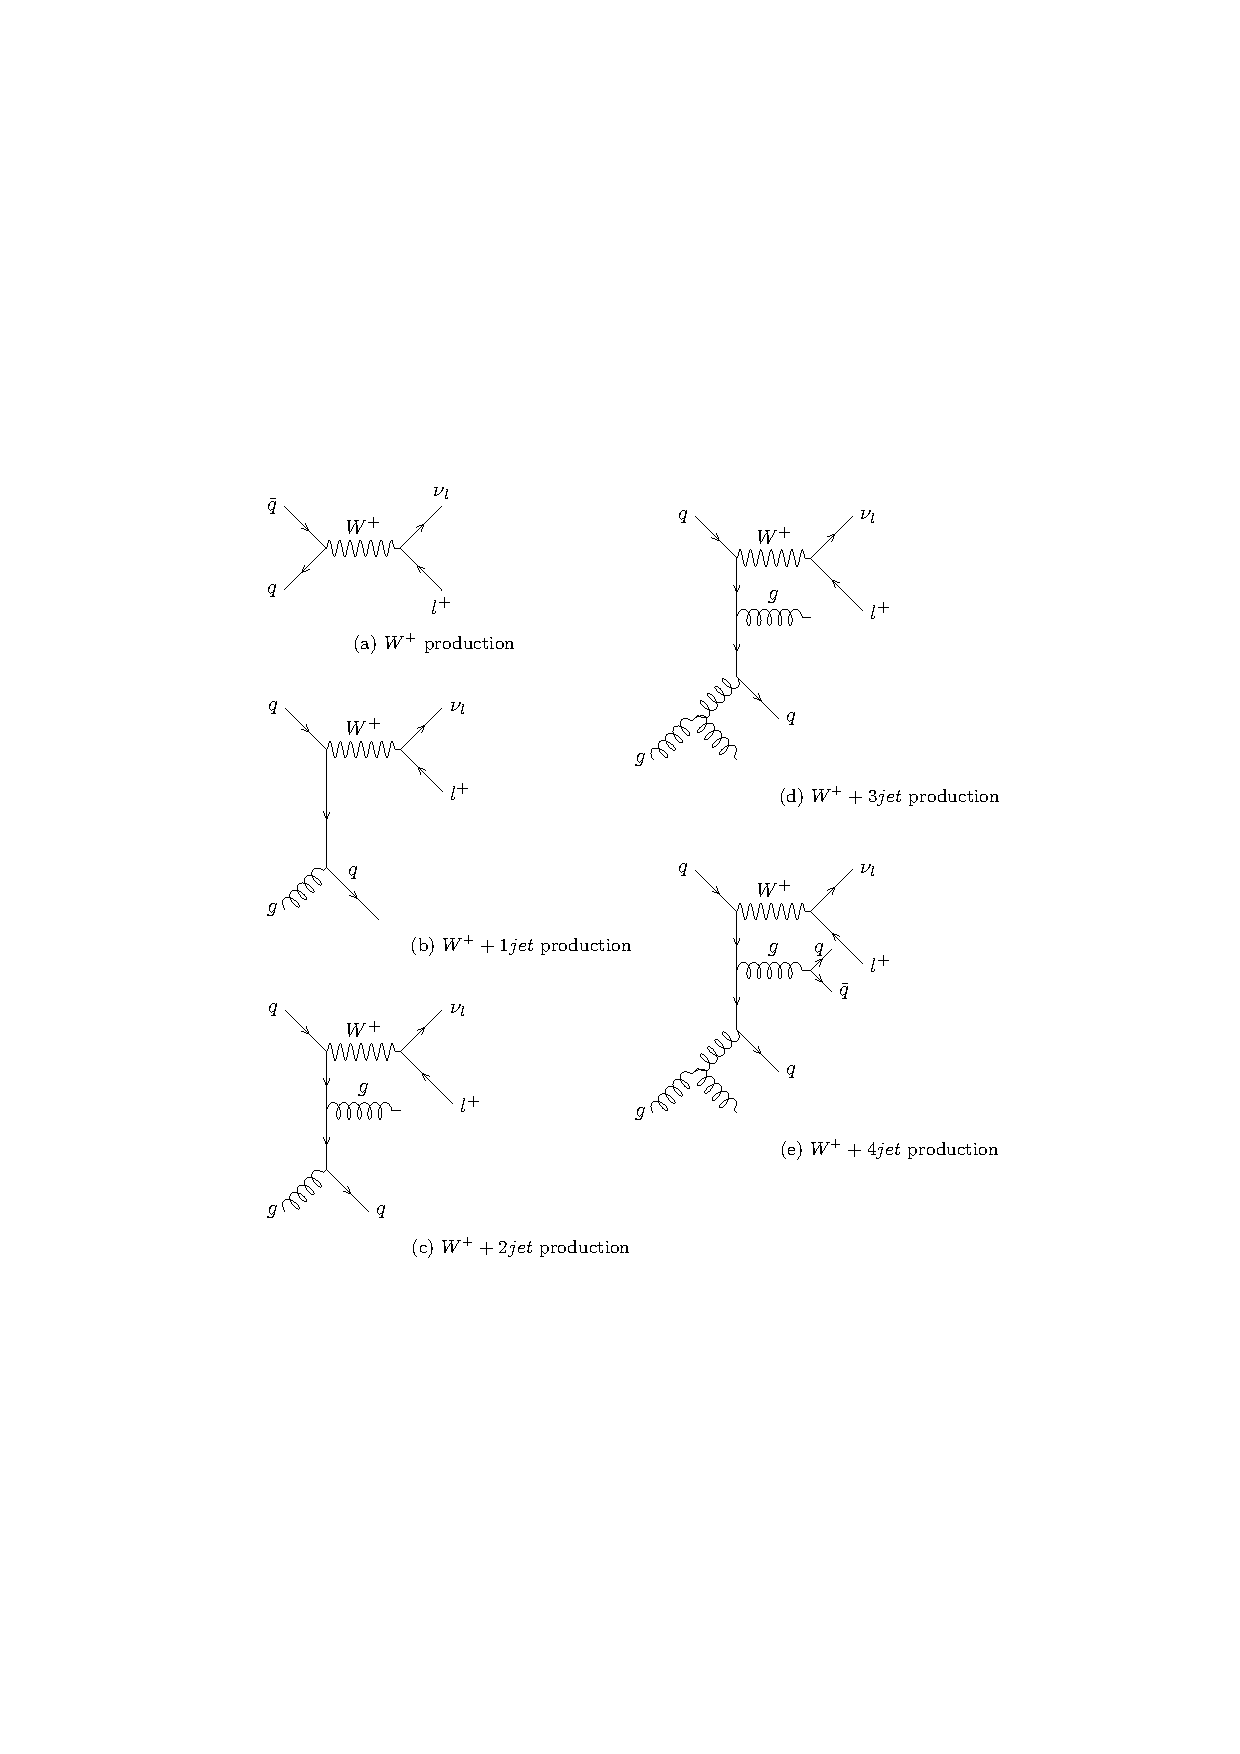
\includegraphics[width=0.75\textwidth]{Image/FeynDiag/feyn_diag_wjet.pdf}
	\caption{Representative Feynman diagrams for $\PW + \rm{n jets}$ channel. The 
	\PW boson is produced by quark-quark and quark-gluon scattering 
	along with n jets (n = 0, 1, 2, 3, 4).}
	\label{fig:feyn_diag_wjet}
	\end{center}
	\end{figure}

\item ${\bf{Z/}}$$\gamma$ ${\bf{+ jets}}$: The Drell-Yan processes in which 
	$Z/\gamma$ are produced along with jets, have lepton and jets at parton level as 
	shown in Figure~\ref{fig:feyn_diag_dyjet}. However, after the 
	reconstruction, the \MET is also found in the events due to the poor 
	measurement of energy in the detector.
	\begin{enumerate}[leftmargin=*]
  	\item $Z/\gamma +\rm{ jets   }(Z/\gamma \rightarrow l^+ l^-)$
  	\item $Z/\gamma +\rm{ 1 jet  }(Z/\gamma \rightarrow l^+ l^-)$
  	\item $Z/\gamma +\rm{ 2 jets }(Z/\gamma \rightarrow l^+ l^-)$
  	\item $Z/\gamma +\rm{ 3 jets }(Z/\gamma \rightarrow l^+ l^-)$
  	\item $Z/\gamma +\rm{ 4 jets }(Z/\gamma \rightarrow l^+ l^-)$
  	\end{enumerate}
	\begin{figure}
	\begin{center}
	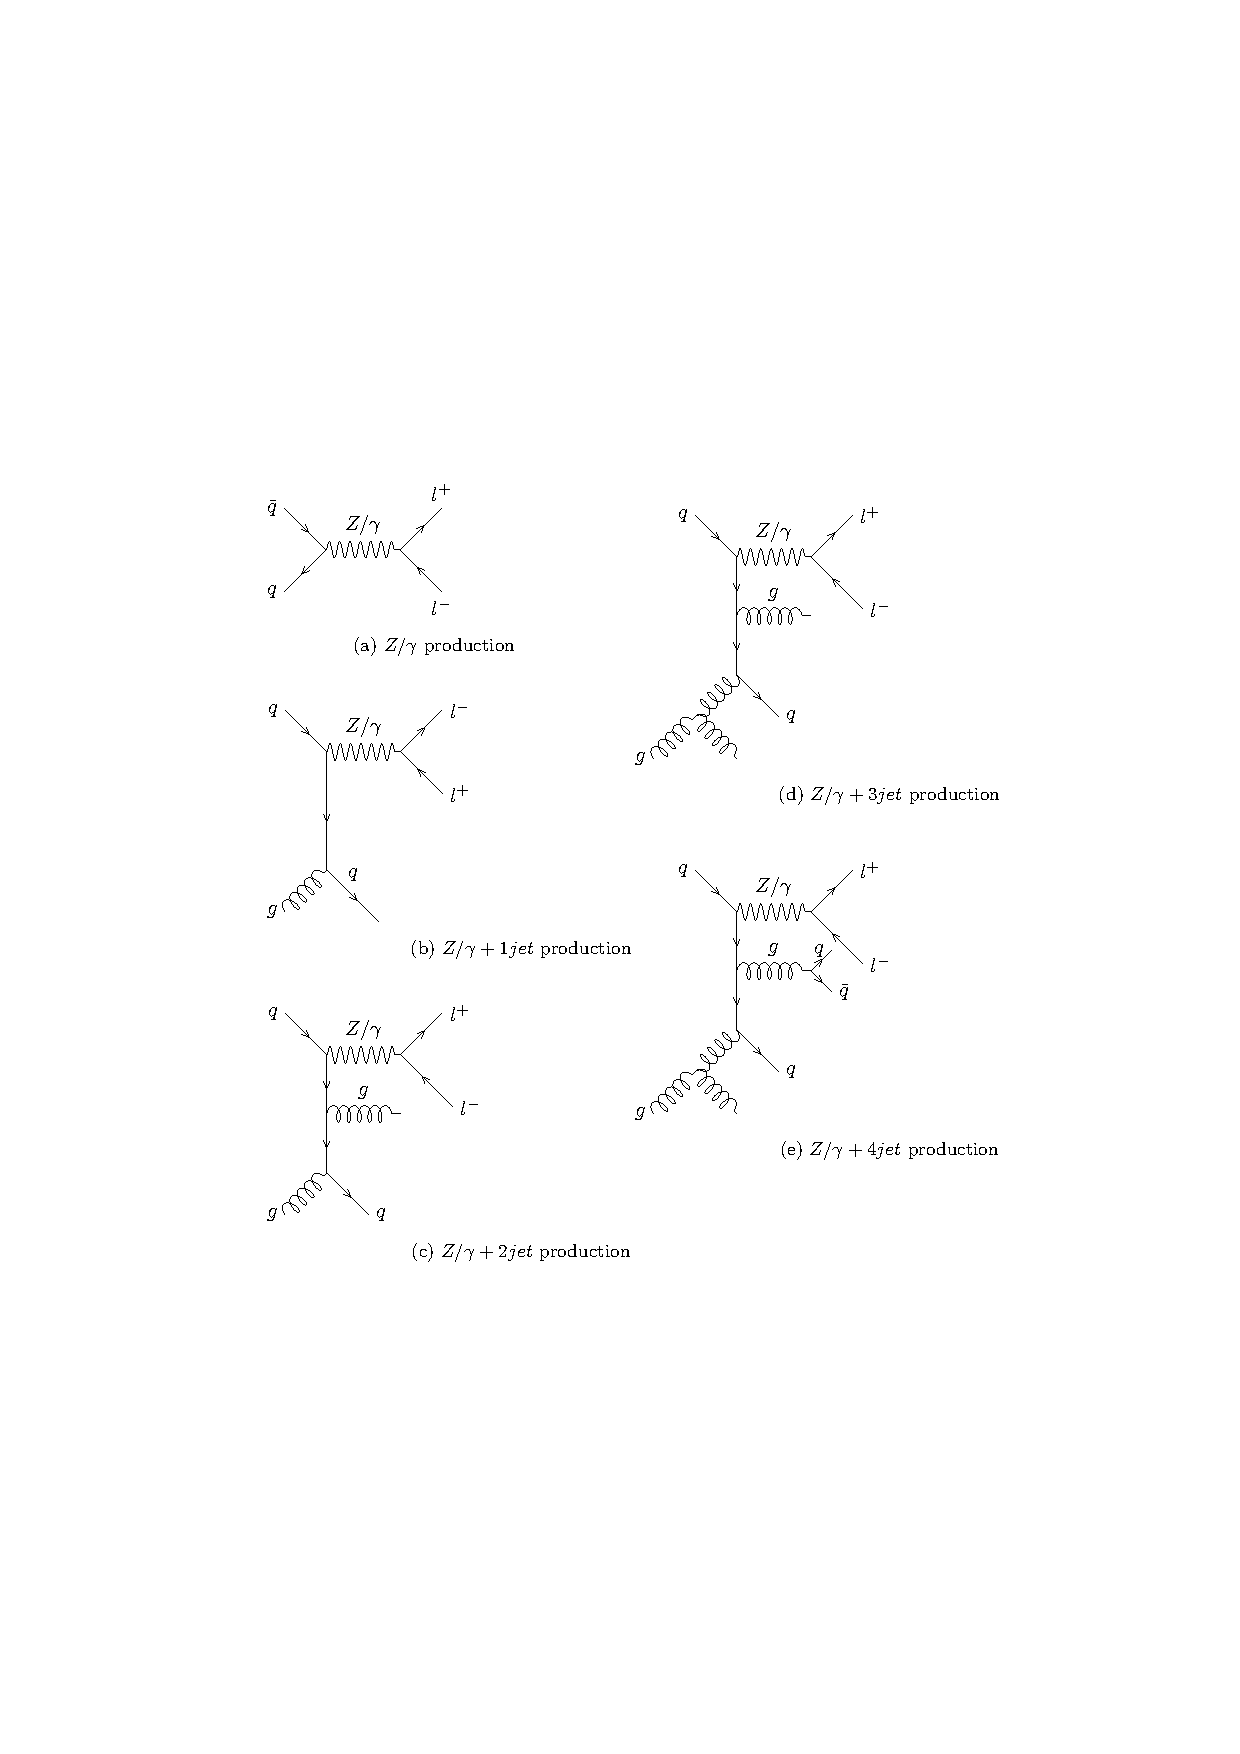
\includegraphics[width=0.75\textwidth]{Image/FeynDiag/feyn_diag_dyjet.pdf}
	\caption{Representative Feynman diagrams for $ Z/\gamma + \rm{n jets}$ channel. 
	The $Z/\gamma$ is produced by quark-quark and quark-gluon scattering 
	along with n jets (n = 0, 1, 2, 3, 4).}
	\label{fig:feyn_diag_dyjet}
	\end{center}
	\end{figure}

\item {\bf{VV}}: Vector boson fusion processes are the smallest background in the signal 
	search region. The fusion happens via tri-linear coupling between the 
	$W^\pm$ and \PZ. The \PZ boson further decays to $l^+l^-$. The vector boson pair production process (VV) has 
	three sub-categories: WW, WZ, and ZZ.
\end{enumerate}

